\documentclass[compress]{beamer}

\mode<presentation> {
  \usetheme{Berlin}

  \setbeamercovered{transparent}
}

\usepackage{default}
\usepackage{listings}
\usepackage{color}

\definecolor{ColorCodeBackground}{rgb}{0.7,0.7,0.7} 

\lstset{language=C++,backgroundcolor=\color{ColorCodeBackground},
basicstyle=\small,numbers=left}

\title{Jafar, a C/C++ interactive development environnement}
\author{Cyrille Berger}

\AtBeginSection[] {
  \begin{frame}<beamer>
    \tableofcontents[currentsection]
  \end{frame}
}

\begin{document}

\begin{frame}
  \titlepage
\end{frame}

\begin{frame}
  \frametitle{Content of the coure}
  \tableofcontents
\end{frame}

%%%%%%%%%%%%%%%%%%%%%%%%%%%%%%%%%%%%%%%%%%%%%%%%%%%%%%%%%%%%%%%%%%%%%%%%%%%%%%%%
%%%%%%%%%%%%%%%%%%%%%%%%%%%%%%%%%%%%%%%%%%%%%%%%%%%%%%%%%%%%%%%%%%%%%%%%%%%%%%%%
%%%%%%%%%%%%%%%%%%%%%%%%%%%%%%%%%%%%%%%%%%%%%%%%%%%%%%%%%%%%%%%%%%%%%%%%%%%%%%%%

\section{What is Jafar ?}
\begin{frame}
  \frametitle{Main Goals}
  \begin{itemize}
   \item<1-> Sharing: don't reinvent the wheel ?
    \begin{itemize}
     \item<2-> Algorithms
     \item<3-> Visualisation, data access...
    \end{itemize}
   \item<4-> Ease the development
  \end{itemize}
\end{frame}

\begin{frame}
 \frametitle{Main features}
 \begin{itemize}
  \item<1-> Support for C/C++
  \item<2-> A build system
  \item<3-> Interactive shell, tcl or ruby
  \item<4-> Modular environnement
  \item<5-> Bindings with swig
  \item<6-> Errors reporting
  \item<7-> Unit testing
  \item<8-> Documentation
 \end{itemize}
\end{frame}

\begin{frame}
 \frametitle{Jafar and Genom}
 \begin{itemize}
  \item<1-> Very similar: modules, interractive shell...
  \item<2-> Genom is for integration on Robot => very few visible
functionnality
  \item<3-> Jafar is for developement => everything should be visible
 \end{itemize}
\end{frame}

\begin{frame}
 \frametitle{Jafar Structure}
 \begin{itemize}
  \item<1-> Directories
    \begin{itemize}
     \item<2-> bin : various tools
     \item<3-> modules : all the installed modules
     \item<4-> doc : the documentation
    \end{itemize}
  \item<5-> Subversion layout
    \begin{itemize}
     \item<6-> svn+ssh://svn.laas.fr/svn/jafar/jafarBackbone/trunk/ : the heart
of jafar
     \item<7-> svn+ssh://cberger@svn.laas.fr/svn/jafar/jafarModules/trunk/ :
all the modules
    \end{itemize}
 \end{itemize}
\end{frame}

%%%%%%%%%%%%%%%%%%%%%%%%%%%%%%%%%%%%%%%%%%%%%%%%%%%%%%%%%%%%%%%%%%%%%%%%%%%%%%%%
%%%%%%%%%%%%%%%%%%%%%%%%%%%%%%%%%%%%%%%%%%%%%%%%%%%%%%%%%%%%%%%%%%%%%%%%%%%%%%%%
%%%%%%%%%%%%%%%%%%%%%%%%%%%%%%%%%%%%%%%%%%%%%%%%%%%%%%%%%%%%%%%%%%%%%%%%%%%%%%%%

\section{What is a Jafar Module ?}
\begin{frame}
  \frametitle{A Jafar module is...}
  \begin{itemize}
   \item<1-> A C/C++ library
   \item<2-> A set of tcl/ruby scripts
   \item<3-> Documentation
   \item<4-> Unit tests
  \end{itemize}
\end{frame}
\begin{frame}
  \frametitle{Directory structure}
  \begin{center}
    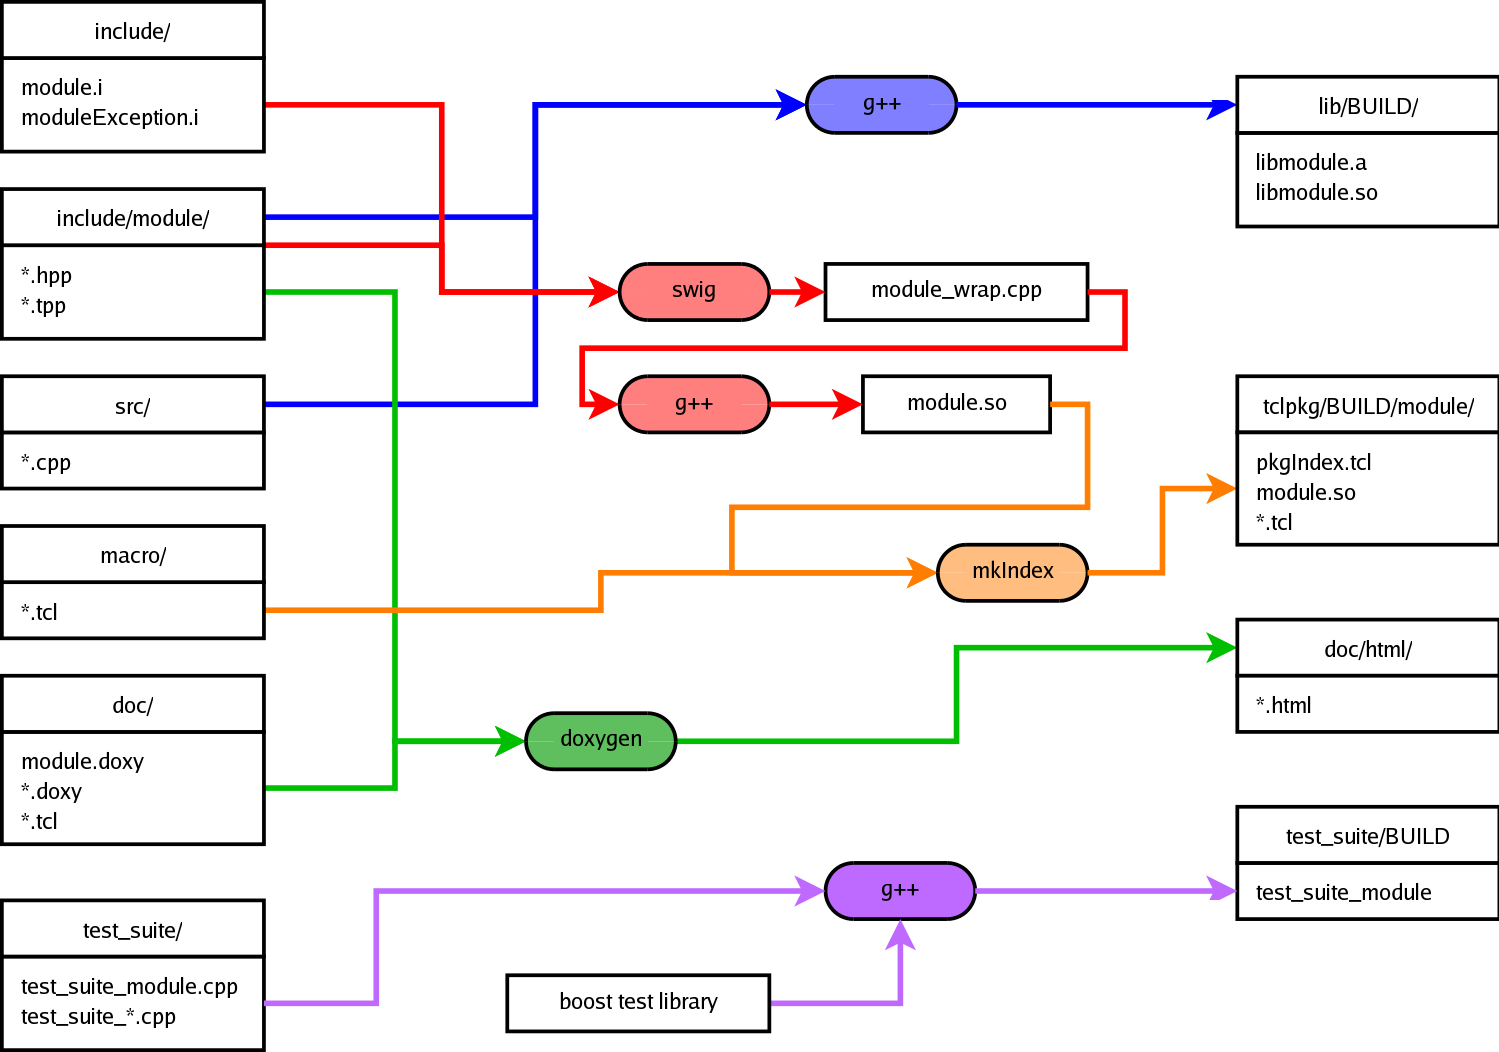
\includegraphics[width=0.9\textwidth]{jafarModule.png}
  \end{center}
\end{frame}

\begin{frame}[fragile]
  \frametitle{How to create a module ?}
  \begin{lstlisting}
cd ${JAFAR_DIR}/modules
../bin/jafar-module -c playmodule
  \end{lstlisting}
\end{frame}

\begin{frame}
  \frametitle{A tour inside the new module}
  \begin{itemize}
   \item<1-> User.make
   \item<2-> include/playmodule.i
   \item<3-> include/playmoduleException.hpp
   \item<4-> src/playmoduleException.cpp
   \item<5-> macro/
   \item<6-> test\_suite/
   \item<7-> doc/
  \end{itemize}
\end{frame}

\begin{frame}
  \frametitle{Important options in User.make}
  \begin{itemize}
   \item<1-> \textit{CPPFLAGS += -DJFR\_NDEBUG} : disable debug output/checking
in jafar
   \item<2-> \textit{CPPFLAGS += -DNDEBUG} : disable debug output/checking
in most external libraries (such as boost)
   \item<3-> \textit{CXXFLAGS += -O2} : force optimisation in the module
  \end{itemize}
\end{frame}


\section{First steps with the new module}
\begin{frame}[fragile]
  \frametitle{Compilation}
  \begin{itemize}
    \item<1-> Compile it
      \begin{lstlisting}[language=bash]
make
      \end{lstlisting}
    \item<2-> Load it
      \begin{lstlisting}[language=ruby]
require 'jafar/playmodule'
      \end{lstlisting}
    \item<3-> So what is available...
  \end{itemize}
\end{frame}

\begin{frame}[fragile]
  \frametitle{A first class: header}
  \begin{lstlisting}
#ifndef _MY_FIRST_CLASS_
#define _MY_FIRST_CLASS_
namespace jafar {
  namespace playmodule {
    class MyFirstClass {
      public:
        int add(int u, int v) const;
    };
  }
}
#endif
  \end{lstlisting}
\end{frame}

\begin{frame}[fragile]
  \frametitle{A first class: source}
  \begin{lstlisting}
#include "playmodule/MyFirstClass.hpp"

using namespace jafar::playmodule;

int MyFirstClass::add(int u, int v) const
{
  return u + v;
}
  \end{lstlisting}
\end{frame}

\begin{frame}[fragile]
  \frametitle{Bind it}
  Open file \textit{playmodule.i} and add:
  \begin{lstlisting}
#include "playmodule/MyFirstClass.hpp"
  \end{lstlisting}
  And:
  \begin{lstlisting}
%include "playmodule/MyFirstClass.i"
  \end{lstlisting}
\end{frame}

\begin{frame}[fragile]
  \frametitle{Use it}
  \begin{lstlisting}
require 'jafar/playmodule'
obj = Playmodule::MyFirstClass.new
obj.add( 1, 2)
  \end{lstlisting}
\end{frame}

%%%%%%%%%%%%%%%%%%%%%%%%%%%%%%%%%%%%%%%%%%%%%%%%%%%%%%%%%%%%%%%%%%%%%%%%%%%%%%%%
%%%%%%%%%%%%%%%%%%%%%%%%%%%%%%%%%%%%%%%%%%%%%%%%%%%%%%%%%%%%%%%%%%%%%%%%%%%%%%%%
%%%%%%%%%%%%%%%%%%%%%%%%%%%%%%%%%%%%%%%%%%%%%%%%%%%%%%%%%%%%%%%%%%%%%%%%%%%%%%%%

\section{Durable code developement}

\begin{frame}
  \frametitle{What are unit tests ?}
  From wikipedia: \textit{In computer programming, unit testing is a method of
testing that verifies the individual units of source code are working properly.}

  \begin{itemize}
    \item<1-> Test the behavior of individual functions
    \item<2-> As much as possible independent tests
    \item<3-> Automatic
  \end{itemize}

\end{frame}

\begin{frame}
  \frametitle{Why unit tests are important ?}
  \begin{itemize}
    \item<1-> Make sure your code does what you want it to do
    \item<2-> Speed up development and optimizations/refactoring
    \item<3-> Make sure nobody else breaks your feature
    \item<4-> Tests are documentation
  \end{itemize}

\end{frame}

\begin{frame}[fragile]
  \frametitle{Write an unit test.}
  Add a file test\_suite/test\_MyFirstClass.cpp :
  \begin{lstlisting}
#include <boost/test/auto_unit_test.hpp>
#include <kernel/jafarTestMacro.hpp>
#include "playmodule/MyFirstClass.hpp"

BOOST_AUTO_TEST_CASE( test_MyFirstClass )
{
  MyFirstClass mfc;
  JFR_CHECK_EQUAL( mfc.add(1, 2), 3 );
}
  \end{lstlisting}
  Then:
  \begin{lstlisting}
make test
  \end{lstlisting}
  
\end{frame}

\begin{frame}
  \frametitle{Documentation: a brief introduction to doxygen}
  Generatl tags:
  \begin{itemize}
    \item \textbf{@ingroup} declare a function to be part of a group
    \item \textbf{@ref} give a reference to an other function/class
  \end{itemize}

  Function tags:
  \begin{itemize}
    \item \textbf{@param} describe a parameter
    \item \textbf{@return} describe the return parameter
  \end{itemize}

\end{frame}

\begin{frame}[fragile]
  \frametitle{Lets document MyFirstClass}
  \begin{lstlisting}
/**
 * This is my first class in Jafar. @ref add is
 * the most important function.
 * @ingroup playmodule
 */
class MyFirstClass {
  public:
    /**
     * This function add two numbers.
     * @param u first number
     * @param v second number
     * @return the addition of u with v
     */
    int add(int u, int v) const;
};
  \end{lstlisting}
\end{frame}

%%%%%%%%%%%%%%%%%%%%%%%%%%%%%%%%%%%%%%%%%%%%%%%%%%%%%%%%%%%%%%%%%%%%%%%%%%%%%%%%
%%%%%%%%%%%%%%%%%%%%%%%%%%%%%%%%%%%%%%%%%%%%%%%%%%%%%%%%%%%%%%%%%%%%%%%%%%%%%%%%
%%%%%%%%%%%%%%%%%%%%%%%%%%%%%%%%%%%%%%%%%%%%%%%%%%%%%%%%%%%%%%%%%%%%%%%%%%%%%%%%
%%%%%%%%%%%%%%%%%%%%%%%%%%%%%%%%%%%%%%%%%%%%%%%%%%%%%%%%%%%%%%%%%%%%%%%%%%%%%%%%
%%%%%%%%%%%%%%%%%%%%%%%%%%%%%%%%%%%%%%%%%%%%%%%%%%%%%%%%%%%%%%%%%%%%%%%%%%%%%%%%
%%%%%%%%%%%%%%%%%%%%%%%%%%%%%%%%%%%%%%%%%%%%%%%%%%%%%%%%%%%%%%%%%%%%%%%%%%%%%%%%

\section{Modules}

%%%%%%%%%%%%%%%%%%%%%%%%%%%%%%%%%%%%%%%%%%%%%%%%%%%%%%%%%%%%%%%%%%%%%%%%%%%%%%%%
%%%%%%%%%%%%%%%%%%%%%%%%%%%%%%%%%%%%%%%%%%%%%%%%%%%%%%%%%%%%%%%%%%%%%%%%%%%%%%%%
%%%%%%%%%%%%%%%%%%%%%%%%%%%%%%%%%%%%%%%%%%%%%%%%%%%%%%%%%%%%%%%%%%%%%%%%%%%%%%%%

\subsection{kernel}

\begin{frame}
  \frametitle{Features}
  \begin{itemize}
   \item Debug
   \item Usefull macros
   \item Configuration file
   \item Timing tool
  \end{itemize}
\end{frame}

%%%%%%%%%%%%%%%%%%%%%%%%%%%%%%%%%%%%%%%%%%%%%%%%%%%%%%%%%%%%%%%%%%%%%%%%%%%%%%%%

\begin{frame}[fragile]
  \frametitle{Debug (1/2)}
  \begin{itemize}
    \item<1-> DataLogger : to log data into a file
    \item<2-> Debug macro : JFR\_DEBUG
      \begin{lstlisting}
  JFR_DEBUG( u << " + " << v << " = " << (u+v) );
      \end{lstlisting}
      Disable debug:
      \begin{lstlisting}
  Jafar::Kernel::DebugStream::moduleOff("playmodule");
      \end{lstlisting}
  \end{itemize}
\end{frame}

\begin{frame}[fragile]
  \frametitle{Debug (2/2)}
  \begin{itemize}
   \item JFR\_ASSERT / JFR\_PRED\_ERROR : check that a parameter is correct
      \begin{lstlisting}
int MyFirstClass::div(int u, int v) const
{
  JFR_ASSERT( v != 0, "Can't divide by 0");
  return u / v;
}
      \end{lstlisting}
  \end{itemize}
\end{frame}

%%%%%%%%%%%%%%%%%%%%%%%%%%%%%%%%%%%%%%%%%%%%%%%%%%%%%%%%%%%%%%%%%%%%%%%%%%%%%%%%

\begin{frame}[fragile]
  \frametitle{Usefull macros}
  For instance JFR\_FOREACH:
  \begin{lstlisting}
std::vector< CoolObject > coolObjects;
JFR_FOREACH( CoolObject& coolObject, coolObjects )
{
  coolObject.soSomethingCool();
}
  \end{lstlisting}
  Instead of:
  \begin{lstlisting}
std::vector< CoolObject > coolObjects;
for( std::vector< CoolObject >::iterator it
     = coolObjects.begin();
  it = coolObjects.end(); ++it )
{
  it->soSomethingCool();
}
  \end{lstlisting}
\end{frame}

%%%%%%%%%%%%%%%%%%%%%%%%%%%%%%%%%%%%%%%%%%%%%%%%%%%%%%%%%%%%%%%%%%%%%%%%%%%%%%%%

\begin{frame}[fragile]
  \frametitle{Configuration file (1/3)}
Exemple of configuration file:
\begin{lstlisting}
MyValue: 10
OtherValue: hello
\end{lstlisting}
  
Exemple of code to read file:
\begin{lstlisting}
KeyValueFile configFile;
configFile.readFile( "test.cfg");
int val;
configFile.getItem( "MyValue", val );
std::string val2;
configFile.getItem( "OtherValue", val2 );
\end{lstlisting}


\end{frame}

%%%%%%%%%%%%%%%%%%%%%%%%%%%%%%%%%%%%%%%%%%%%%%%%%%%%%%%%%%%%%%%%%%%%%%%%%%%%%%%%

\begin{frame}[fragile]
  \frametitle{Configuration file (2/3)}
KeyValueFileSave: an object which can save its parameters.
 
\begin{lstlisting}
class CoolAlgorithm : public KeyValueFileSave {
  public:
    virtual void saveKeyValueFile(
    jafar::kernel::KeyValueFile& keyValueFile)
    {
      keyValueFile.setItem("MyParameter", m_parameter );
    }
  public:
    int m_parameter;
};

CoolAlgorithm coolAlgorithm;
coolAlgorithm.save("algo.cfg");

\end{lstlisting}
 
\end{frame}

%%%%%%%%%%%%%%%%%%%%%%%%%%%%%%%%%%%%%%%%%%%%%%%%%%%%%%%%%%%%%%%%%%%%%%%%%%%%%%%%

\begin{frame}[fragile]
  \frametitle{Configuration file (3/3)}
KeyValueFileLoad: an object which can load its parameters.
 
\begin{lstlisting}
class CoolAlgorithm : public KeyValueFileLoad {
  public:
    virtual void loadKeyValueFile(
    jafar::kernel::KeyValueFile const& keyValueFile)
    {
      keyValueFile.getItem("MyParameter", m_parameter );
    }
  public:
    int m_parameter;
};

CoolAlgorithm coolAlgorithm;
coolAlgorithm.load("algo.cfg");
\end{lstlisting}
 
\end{frame}

%%%%%%%%%%%%%%%%%%%%%%%%%%%%%%%%%%%%%%%%%%%%%%%%%%%%%%%%%%%%%%%%%%%%%%%%%%%%%%%%

\begin{frame}[fragile]
  \frametitle{Timing tools}
  \begin{itemize}
    \item<1-> Chrono
\begin{lstlisting}
 Chrono chrono;
 chrono.start();
 // Do some extensive computation
 JFR_DEBUG(chrono.elapsed());
\end{lstlisting}
    \item<2-> Framerate
  \end{itemize}

\end{frame}

%%%%%%%%%%%%%%%%%%%%%%%%%%%%%%%%%%%%%%%%%%%%%%%%%%%%%%%%%%%%%%%%%%%%%%%%%%%%%%%%
%%%%%%%%%%%%%%%%%%%%%%%%%%%%%%%%%%%%%%%%%%%%%%%%%%%%%%%%%%%%%%%%%%%%%%%%%%%%%%%%
%%%%%%%%%%%%%%%%%%%%%%%%%%%%%%%%%%%%%%%%%%%%%%%%%%%%%%%%%%%%%%%%%%%%%%%%%%%%%%%%

\subsection{jmath}
\begin{frame}
  \frametitle{Features}
  \begin{itemize}
   \item matrix and vectors computation
   \item use lapack
   \item linear solvers
   \item least-square optimization
  \end{itemize}
\end{frame}

%%%%%%%%%%%%%%%%%%%%%%%%%%%%%%%%%%%%%%%%%%%%%%%%%%%%%%%%%%%%%%%%%%%%%%%%%%%%%%%%

\begin{frame}[fragile]
  \frametitle{Create vectors and matrix}
  \begin{itemize}
   \item<1-> Bounded vectors
   \begin{onlyenv}<1-1>
   \begin{lstlisting}
jblas::vec2 vec_2;
jblas::vec3 vec_3;
jblas::vec4 vec_4;
   \end{lstlisting}
   \end{onlyenv}
   \item<2-> Unbounded vectors
    \begin{onlyenv}<2-2>
      \begin{lstlisting}
jblas::vec vec_n( 10 );
      \end{lstlisting}
    \end{onlyenv}
   \item<3-> Bounded matrix
    \begin{onlyenv}<3-3>
      \begin{lstlisting}
jblas::mat22 mat_22;
jblas::mat33 mat_33;
jblas::mat44 mat_44;
      \end{lstlisting}
    \end{onlyenv}
   \item<4-> Unbounded matrix
    \begin{onlyenv}<4-4>
      \begin{lstlisting}
jblas::mat mat_nn(100,400);
      \end{lstlisting}
    \end{onlyenv}
    \item<5-> Zero, Scalar and Identity matrix
    \begin{onlyenv}<5-5>
      \begin{lstlisting}
jblas::mat mat = jblas::zero_mat(5);
jblas::mat mat = jblas::identity_mat(5);
jblas::mat mat = 5.0 * jblas::scalar_mat(5); // Matrix filled with 5.0
      \end{lstlisting}
    \end{onlyenv}
  \end{itemize}
\end{frame}

%%%%%%%%%%%%%%%%%%%%%%%%%%%%%%%%%%%%%%%%%%%%%%%%%%%%%%%%%%%%%%%%%%%%%%%%%%%%%%%%

\begin{frame}[fragile]
  \frametitle{Vectors and matrix operations}
  \begin{itemize}
   \item<1-> Addition, substraction
    \begin{onlyenv}<1-1>
      \begin{lstlisting}
jblas::vec2 v1, v2, v3;
v1 = v1 + v2 - v3;
      \end{lstlisting}
    \end{onlyenv}
   \item<2-> Multiplication
    \begin{onlyenv}<2-2>
      \begin{lstlisting}
jblas::mat m1, m2, m3;
m3 = ublas::prod( m1, m2 );
m3 = ublas::prod( m1,
jblas::mat( ublas::prod( m3, m2 ) );
      \end{lstlisting}
    \end{onlyenv}
    \item<3-> Transposition
    \begin{onlyenv}<3-3>
      \begin{lstlisting}
jblas::mat m4 = ublas::trans(m3);
m4 = ublas::prod( ublas::trans(m2), m1 );
      \end{lstlisting}
    \end{onlyenv}
    \item<4-> Inversion
    \begin{onlyenv}<4-4>
      \begin{lstlisting}
ublasExtra::inv( m4 );
      \end{lstlisting}
    \end{onlyenv}
    \item<5-> Dot and cross product
    \begin{onlyenv}<5-5>
      \begin{lstlisting}
ublas::outer_prod( v1, v2 ); // cross product
ublas::inner_prod( v1, v2 ); // dot product
      \end{lstlisting}
    \end{onlyenv}
    \item<6-> Determinant
    \begin{onlyenv}<6-6>
      \begin{lstlisting}
ublasExtra::det( m4 );
      \end{lstlisting}
    \end{onlyenv}
  \end{itemize}
\end{frame}

%%%%%%%%%%%%%%%%%%%%%%%%%%%%%%%%%%%%%%%%%%%%%%%%%%%%%%%%%%%%%%%%%%%%%%%%%%%%%%%%

\begin{frame}[fragile]
  \frametitle{Symmetric matrix}
  \begin{itemize}
   \item<1-> Bounded symmetric matrix:
    \begin{onlyenv}<1-1>
      \begin{lstlisting}
jblas::sym_mat22 mat_22;
jblas::sym_mat33 mat_33;
jblas::sym_mat44 mat_44;
      \end{lstlisting}
    \end{onlyenv}
   \item<2-> Unbounded symmetric matrix:
    \begin{onlyenv}<2-2>
      \begin{lstlisting}
jblas::sym_mat mat_nn(100);
      \end{lstlisting}
    \end{onlyenv}
   \item<3-> Create symmetrix matrix from non symmetric matrix
    \begin{onlyenv}<3-3>
      \begin{lstlisting}
jblas::sym mat_nn(100);
jblas::sym_mat smat_nn =
    ublas::symmetric_adaptor<jblas::mat44,
        ublas::lower>( mat_nn );
jblas::sym_mat smat_nn =
    ublas::symmetric_adaptor<jblas::mat44,
        ublas::upper>( mat_nn );
      \end{lstlisting}
    \end{onlyenv}
   \item<4-> Access elements
    \begin{onlyenv}<4-4>
      \begin{lstlisting}
jblas::sym_mat22 mat_22;
mat_22(0,1) = 10.0;
// Warning:
mat_22(1,0) = 12.0;
JFR_DEBUG( mat_22(1,0) ); // will display 10.0 !
      \end{lstlisting}
    \end{onlyenv}
  \end{itemize}

\end{frame}

%%%%%%%%%%%%%%%%%%%%%%%%%%%%%%%%%%%%%%%%%%%%%%%%%%%%%%%%%%%%%%%%%%%%%%%%%%%%%%%%

\begin{frame}[fragile]
  \frametitle{Use lapack}
  \begin{itemize}
   \item<1-> To compute SVD and eigen values
   \item<2-> Warning: use column major with Lapack
      \begin{lstlisting}
jblas::mat A( 30, 3 );
jblas::mat_column_major m_A( A );
jblas::vec s(3);
jblas::mat_column_major U(30, 3);
jblas::mat_column_major VT(3, 3);

int ierr = lapack::gesdd(m_A,s,U,VT);
      \end{lstlisting}
  \end{itemize}
\end{frame}


%%%%%%%%%%%%%%%%%%%%%%%%%%%%%%%%%%%%%%%%%%%%%%%%%%%%%%%%%%%%%%%%%%%%%%%%%%%%%%%%

\begin{frame}[fragile]
  \frametitle{Linear least square}
  \begin{itemize}
    \item<1-> Find $ x $ that minimize $ \left\| A.x - b \right\|^2 $
    \item<2-> LinearLeastSquares
      \begin{onlyenv}<2-2>
        \begin{lstlisting}
LinearLeastSquares lls;
lls.setSize( 3 /* model size */,
             10 /* number of points */ );
jblas::vec valueOfA;
double valueOfB;
lls.setData( 0 /* index of point */,
             valueOfA,
             valueOfB );
...
lls.solve();
lls.x(); // return the value of x
lls.xCov(); // return the covariance
        \end{lstlisting}
      \end{onlyenv}
    \item<3-> VariableSizeLinearLeastSquares
      \begin{onlyenv}<3-3>
        \begin{lstlisting}
VariableSizeLinearLeastSquares vsll
            ( 3 /* model size */ );
jblas::vec valueOfA;
double valueOfB;
vsll.addMeasure( valueOfA, valueOfB );
...
vsll.solve();
vsll.x(); // return the value of x
        \end{lstlisting}
      \end{onlyenv}
  \end{itemize}

\end{frame}

%%%%%%%%%%%%%%%%%%%%%%%%%%%%%%%%%%%%%%%%%%%%%%%%%%%%%%%%%%%%%%%%%%%%%%%%%%%%%%%%
%%%%%%%%%%%%%%%%%%%%%%%%%%%%%%%%%%%%%%%%%%%%%%%%%%%%%%%%%%%%%%%%%%%%%%%%%%%%%%%%
%%%%%%%%%%%%%%%%%%%%%%%%%%%%%%%%%%%%%%%%%%%%%%%%%%%%%%%%%%%%%%%%%%%%%%%%%%%%%%%%

\subsection{geom}
\begin{frame}
  \frametitle{Features}
  \begin{itemize}
   \item<1-> T3D: 3D Transformation
   \item<2-> Geometric classes such as Point, Lines, Boxes...
  \end{itemize}
\end{frame}

\begin{frame}[fragile]
  \frametitle{T3D: 3D Transformation}
  \begin{itemize}
    \item<1-> Support for Euler and Quaternion
      \begin{onlyenv}<1-1>
        \begin{lstlisting}
jblas::vec transfoX(6);
transfoX(0) = x;
transfoX(1) = y;
transfoX(2) = z;
transfoX(3) = yaw;
transfoX(4) = pitch;
transfoX(5) = roll;
geom::T3DEuler transfo( transfoX );
        \end{lstlisting}
      \end{onlyenv}
    \item<2-> Composition
      \begin{onlyenv}<2-2>
        \begin{lstlisting}
geom::T3DEuler robotToWorld = something;
geom::T3DEuler sensorToRobot = something;
geom::T3DEuler sensorToWorld;
geom::T3D::compose( sensorToRobot, 
                    robotToWorld,
                    sensorToWorld);
        \end{lstlisting}
      \end{onlyenv}
    \item<3-> Invert
      \begin{onlyenv}<3-3>
        \begin{lstlisting}
geom::T3DEuler robotToWorld = something;
geom::T3DEuler worldToRobot;
geom::T3D::invert( robotToWorld, worldToRobot );
        \end{lstlisting}
      \end{onlyenv}
    \item<4-> Transform a vector
      \begin{onlyenv}<4-4>
        \begin{lstlisting}
geom::T3DEuler sensorToWorld = something;
jblas::vec X_sensor;
jblas::vec X_world = ublas::prod( sensorToWorld.getM(), X_sensor );
        \end{lstlisting}
      \end{onlyenv}
    
  \end{itemize}
\end{frame}

%%%%%%%%%%%%%%%%%%%%%%%%%%%%%%%%%%%%%%%%%%%%%%%%%%%%%%%%%%%%%%%%%%%%%%%%%%%%%%%%

\begin{frame}[fragile]
  \frametitle{Geometric classes}
  \begin{itemize}
    \item<1-> Points
      \begin{onlyenv}<1-1>
        \begin{lstlisting}
jblas::vec v = coordinates of the point;
geom::Point<3> p1( 
          new Point<3>::EuclideanDriver( v ) );
        \end{lstlisting}
      \end{onlyenv}
    \item<2-> Lines
      \begin{onlyenv}<2-2>
        \begin{lstlisting}
jblas::vec v = coordinates of the origin;
jblas::vec v = coordinates of the vector director;
geom::Line<3> l1( 
            new Line<3>::EuclideanDriver( v ) );
geom::Point<3> p1;
geom::Point<3> p2;
geom::Line<3> l2(
    new Line<3>::TwoPointsPointerDriver( &p1, &p2 ) );
geom::Line<3> l2(
              new Line<3>::TwoPointsDriver( p1, p2 ) );
        \end{lstlisting}
      \end{onlyenv}
     \item<3-> Segments, polylines, planes, facets...
     \item<4-> Operations
      \begin{onlyenv}<4-4>
        \begin{lstlisting}
geom::distance( p1, p2 );
geom::distance( p1, l2 );
geom::angle( l1, l2 );
        \end{lstlisting}
      \end{onlyenv}
     \item<5-> Bounding box
\begin{onlyenv}<5-5>
  \begin{lstlisting}
geom::Segment segment( {1,1,1}, {-1,-1,-1} );
segment.boundingBox(); // Return {1,1,1}, {-1,-1,-1}
  \end{lstlisting}
\end{onlyenv}
  \end{itemize}
\end{frame}

\begin{frame}[fragile]
  \frametitle{Geometric classes : VoxelSpace (1/2)}

  \begin{lstlisting}
class Object
{
  public:
    Object(const geom::Atom<3>& atom_)
      : m_atom(atom_)
    {
    }
    const geom::Atom<3>& atom() const 
    { return m_atom; }
  private:
    const geom::Atom<3>& m_atom;
};
  \end{lstlisting}
\end{frame}

\begin{frame}[fragile]
  \frametitle{Geometric classes : VoxelSpace (2/2)}

  \begin{lstlisting}
geom::VoxelSpace<dimension, Object,
    geom::AtomBoundingBoxGetter<dimension, Object> >
    voxelSpace;
geom::Point<3> pt;
Object* obj1 = new Object(pt);
voxelSpace.insertObject( obj1 );
geom::Line<3> li;
Object* obj2 = new Object(li);
voxelSpace.insertObject( obj2 );
geom::BoundingBox<3> bb( onePoint, oneAnotherPoint );
std::list<Object*> objects =
                      voxelSpace.objectsIn( bb );
  \end{lstlisting}

\end{frame}

%%%%%%%%%%%%%%%%%%%%%%%%%%%%%%%%%%%%%%%%%%%%%%%%%%%%%%%%%%%%%%%%%%%%%%%%%%%%%%%%
%%%%%%%%%%%%%%%%%%%%%%%%%%%%%%%%%%%%%%%%%%%%%%%%%%%%%%%%%%%%%%%%%%%%%%%%%%%%%%%%
%%%%%%%%%%%%%%%%%%%%%%%%%%%%%%%%%%%%%%%%%%%%%%%%%%%%%%%%%%%%%%%%%%%%%%%%%%%%%%%%

\subsection{image}
\begin{frame}
  \frametitle{Features}
  \begin{itemize}
   \item<1-> load/read images
   \item<2-> access to the whole OpenCV API
  \end{itemize}
\end{frame}

%%%%%%%%%%%%%%%%%%%%%%%%%%%%%%%%%%%%%%%%%%%%%%%%%%%%%%%%%%%%%%%%%%%%%%%%%%%%%%%%

\begin{frame}[fragile]
  \frametitle{Features}
  \begin{itemize}
   \item<1-> Create an image
\begin{lstlisting}
image::Image dx( width, height, IPL_DEPTH_16S, JfrImage_CS_GRAY );
\end{lstlisting}
    \item<2-> Use a functin from OpenCV
\begin{lstlisting}
image::Image myImage;
myImage.loadImage("MyFile.png");
cvSobel( myImage, dx, 1, 0, 3);
\end{lstlisting}
  \end{itemize}

\end{frame}

%%%%%%%%%%%%%%%%%%%%%%%%%%%%%%%%%%%%%%%%%%%%%%%%%%%%%%%%%%%%%%%%%%%%%%%%%%%%%%%%
%%%%%%%%%%%%%%%%%%%%%%%%%%%%%%%%%%%%%%%%%%%%%%%%%%%%%%%%%%%%%%%%%%%%%%%%%%%%%%%%
%%%%%%%%%%%%%%%%%%%%%%%%%%%%%%%%%%%%%%%%%%%%%%%%%%%%%%%%%%%%%%%%%%%%%%%%%%%%%%%%

\subsection{camera}
\begin{frame}
  \frametitle{Features}
  Camera model:
  \begin{itemize}
   \item Pinhole
   \item Barreto
   \item Stereo bench
  \end{itemize}

\end{frame}

%%%%%%%%%%%%%%%%%%%%%%%%%%%%%%%%%%%%%%%%%%%%%%%%%%%%%%%%%%%%%%%%%%%%%%%%%%%%%%%%
%%%%%%%%%%%%%%%%%%%%%%%%%%%%%%%%%%%%%%%%%%%%%%%%%%%%%%%%%%%%%%%%%%%%%%%%%%%%%%%%
%%%%%%%%%%%%%%%%%%%%%%%%%%%%%%%%%%%%%%%%%%%%%%%%%%%%%%%%%%%%%%%%%%%%%%%%%%%%%%%%

\subsection{datareader}
\begin{frame}
  \frametitle{Features}
  \begin{itemize}
    \item<1-> Read images
    \item<2-> Read positions
  \end{itemize}
\end{frame}
\begin{frame}[fragile]
  \frametitle{Default configuration}
    \begin{itemize}
      \item<1-> set the base directory
        \begin{lstlisting}
Jafar::Datareader::DataReader
    .setDefaultBasePath("/home/cyrille/laas/Data")
        \end{lstlisting}
      \item<2-> set the series name
        \begin{lstlisting}
Jafar::Datareader::DataReader
    .setDefaultSeriesName("pelican")
        \end{lstlisting}
      \item<3-> set the serie number
        \begin{lstlisting}
Jafar::Datareader::DataReader
    .setDefaultSerieNumber(11)
        \end{lstlisting}
    \end{itemize}
\end{frame}

\begin{frame}[fragile]
  \frametitle{Read data}
  \begin{lstlisting}
dr = Datareader::DataReader.new
sr = dr.getStereoReader( 0 )
img = sr.left.loadImage( 0 )
Qdisplay::showimage( img )
  \end{lstlisting}
\end{frame}

%%%%%%%%%%%%%%%%%%%%%%%%%%%%%%%%%%%%%%%%%%%%%%%%%%%%%%%%%%%%%%%%%%%%%%%%%%%%%%%%
%%%%%%%%%%%%%%%%%%%%%%%%%%%%%%%%%%%%%%%%%%%%%%%%%%%%%%%%%%%%%%%%%%%%%%%%%%%%%%%%
%%%%%%%%%%%%%%%%%%%%%%%%%%%%%%%%%%%%%%%%%%%%%%%%%%%%%%%%%%%%%%%%%%%%%%%%%%%%%%%%

\subsection{qdisplay}
\begin{frame}
  \frametitle{Features}
  \begin{itemize}
   \item<1-> display images
   \item<2-> display vectors overlay 
  \end{itemize}
\end{frame}

\begin{frame}[fragile]
  \frametitle{Use}
  \begin{lstlisting}
dr = Datareader::DataReader.new
sr = dr.getStereoReader( 0 )
imgL = sr.left.loadImage( 0 )
imgR = sr.right.loadImage( 0 )

viewer = Jafar::Qdisplay::Viewer.new
imageviewL = Jafar::Qdisplay::ImageView.new(imgL)
viewer.setImageView(imageviewL)
imageviewR = Jafar::Qdisplay::ImageView.new(imgR)
viewer.setImageView(imageviewR, 1, 0)

shape = Qdisplay::Shape.new(Qdisplay::Shape::ShapeRectangle, 10, 10, 5, 5)
shape.setColor(0,255,0)
shape.setLabel("Hello World !")
imageviewL.addShape(shape)
  \end{lstlisting}

\end{frame}

%%%%%%%%%%%%%%%%%%%%%%%%%%%%%%%%%%%%%%%%%%%%%%%%%%%%%%%%%%%%%%%%%%%%%%%%%%%%%%%%
%%%%%%%%%%%%%%%%%%%%%%%%%%%%%%%%%%%%%%%%%%%%%%%%%%%%%%%%%%%%%%%%%%%%%%%%%%%%%%%%
%%%%%%%%%%%%%%%%%%%%%%%%%%%%%%%%%%%%%%%%%%%%%%%%%%%%%%%%%%%%%%%%%%%%%%%%%%%%%%%%

\subsection{And what else ?}
\begin{frame}
  \begin{itemize}
   \item gfm: general feature matching
   \item sift, surf
   \item bundle
   \item stereo
   \item filter : (extended) kalman filter, particle filter
   \item slam
   \item ...
  \end{itemize}

\end{frame}

\end{document}
